\documentclass{udpreport}
%\headertext{Metodos Numéricos}
\title{Metodos Numéricos : Tarea 2}
\author{Thomas Muñoz , Diego Vilches , Javiera Araya , Ignacio Yanjari.}
\usepackage{amssymb}
\usepackage{amsmath}
\usepackage{graphicx}
\usepackage{float}
\usepackage{subfig}
\usepackage{array}
\graphicspath{ {Imagenes/} }
\usepackage{listings}
\usepackage{color}
\providecommand{\norm}[1]{\lVert#1\rVert}

\definecolor{dkgreen}{rgb}{0,0.6,0}
\definecolor{gray}{rgb}{0.5,0.5,0.5}
\definecolor{mauve}{rgb}{0.58,0,0.82}

\lstset{frame=tb,
  language=MATLAB,
  aboveskip=3mm,
  belowskip=3mm,
  showstringspaces=false,
  columns=flexible,
  basicstyle={\small\ttfamily},
  numbers=none,
  numberstyle=\tiny\color{gray},
  keywordstyle=\color{blue},
  commentstyle=\color{dkgreen},
  stringstyle=\color{mauve},
  breaklines=true,
  breakatwhitespace=true,
  tabsize=4
}

\begin{document}
\maketitle
\tableofcontents
\listoffigures
\chapter{Introducción}
El presente informe tiene como objetivo ver  y analizar el funcionamiento de los métodos vistos en catedra, los cuales se centrara en tres ejes fundamentales que son:
\begin{enumerate}
\item Resolución de sistemas lineales.
\item Aproximación de funciones.
\item Integración de funciones. 
\end{enumerate}

En la resolución de sistemas lineales la finalidad es que a lo largo del trabajo se oriente en ocupar métodos con el fin de obtener una solución para determinado sistema para ello se hará uso de diversas factorizaciones como LU o Cholesky,  asi tambien el uso de métodos muy importantes como el de Jacobi o Gauss-Seidel, entre otros, de manera que sea más simple la resolución del sistema. Por otra parte y dentro de este mismo item se verá si una matriz está bien condicionada  y en determinados casos calcular los errores que se pueden dar en  la obtención de soluciones con los métodos utilizados.
En lo que se refiere a aproximación de funciones e integración de funciones, los métodos para interpolar serán el enfoque principal para poder aproximar determinados contornos de figuras específicas, también es importante destacar el uso de la formula el trapecio compuesto que será útil para aproximar integrales definidas.
\newpage

\chapter{Resolución de sistema de ecuaciones lineales} % rellenar con lo que corresponda
 \section{Programación}
 	Sea $A \in \mathbb{R}^{n \times n}$ una matriz invertible y $b \in \mathbb{R}^{n} $. Se considera el siguiente problema:
 	\begin{equation}
 		\textrm{Encontrar un } x \in \mathbb{R}^{n}\textrm{ tal que }  Ax = b
	\end{equation} 	 
	Para solucionarlo, se han programados todos los esquemas directos vistos en clase que pueden ayudar con este objetivo. También se hhan programado las factorizaciones LU,LU con pivoteo parcial y Cholesky de la matriz a. Finalmente, los métodos iterativos: Richardson, Jacobi, Guass-Seidel y SOR. Con un criterio de parada $\frac{\norm{x^{k+1}-x^k}}{\norm{x^k}} \leq Tol_{rel}$
 \section{Aplicación de los esquemas programados}
 \begin{enumerate}
 %%%%%%%%%%%%%%%
 %pregunta 1
 %%%%%%%%%%%%%%%%
 	\item   
 		\begin{enumerate}
 			\item 	
 			\begin{figure}[H]
 				\centering
 				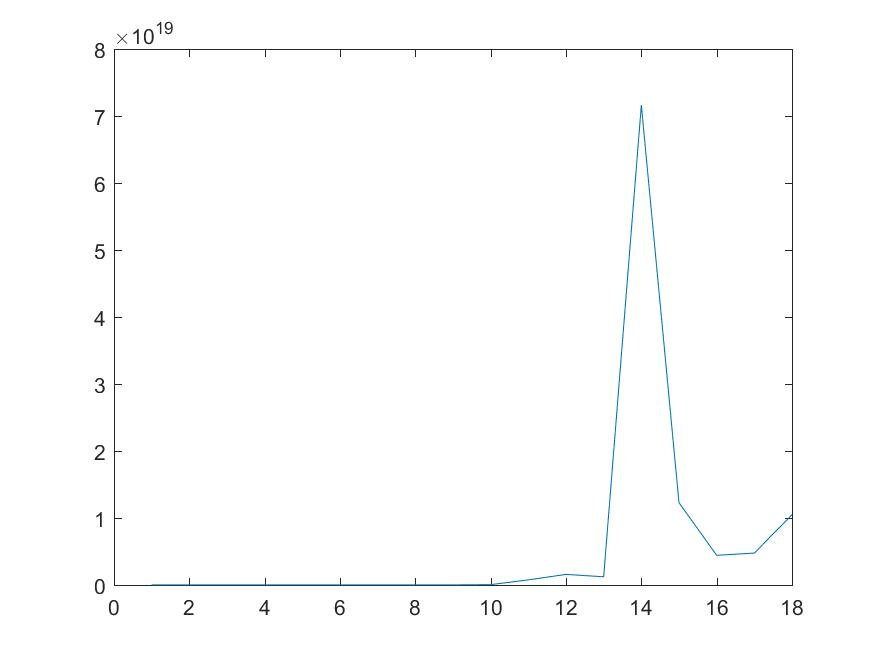
\includegraphics[width=9cm]{grafo1-a}
 				\caption{Gráfico del número de condición para una matriz de Hilbert de tamaño n}
 			\end{figure}
 			Se puede observar en figura 2.1 que entre más grande es el tamaño de la matriz de Hilbert, más grande es su número de condición. Este, al estar significativamente alejado del 1, implica que la matriz está mal condicionada. Esto siginifca, que al ocupar esta matriz como matriz de coeficiente, los resultados obtenidos, no serán tan exactos.  %explica que significa que esté mal condicionada
 			\item 
 				\begin{itemize} 				
 				\item Para n=6:
 				
 				$x_{a} = \left(\begin{array}{c} 1.0\\ 1.0\\ 1.0\\ 1.0\\ 1.0\\ 1.0\\ \end{array}\right)$
 				\\
 				\\
 				\item Para n=10:
 				
 				$x_{a} = \left(\begin{array}{c} 1.0\\ 1.0\\ 1.0\\ 1.0\\ 1.0\\ 1.0\\ 0.9998\\ 1.0\\ 0.9999\\ 1.0 \end{array}\right)$
 				\\
 				\\
 				\item Para n=20:
 				
 				$x_{a} = \left(\begin{array}{c} 1.0\\ 1.0\\ 0.9992\\ 1.008\\ 0.9865\\ 0.6493\\ 4.094\\ -11.3\\ 28.09\\ -30.78\\ 14.27\\ 5.74\\ 8.759\\ -22.04\\ 9.068\\ 0.1336\\ 29.05\\ -42.82\\ 26.48\\ -4.379 \end{array}\right)$
 				\\
 				\\
 				\newpage
 				\item Para n=30:
 				
 				$x_{a} = \left(\begin{array}{c} 1.0\\ 1.0\\ 1.0\\ 0.9929\\ 1.055\\ 0.7579\\ 1.695\\ -0.8953\\ 7.118\\ -14.6\\ 22.59\\ -5.381\\ -19.13\\ 19.89\\ 11.04\\ -26.6\\ 29.17\\ -27.26\\ 32.59\\ -26.64\\ 8.374\\ -8.23\\ 29.33\\ 9.701\\ -39.71\\ -9.034\\ 39.38\\ 2.024\\ -19.37\\ 8.151 \end{array}\right)$
 			\end{itemize}
 			\item 
 			\begin{figure}[H]
 				\centering
 				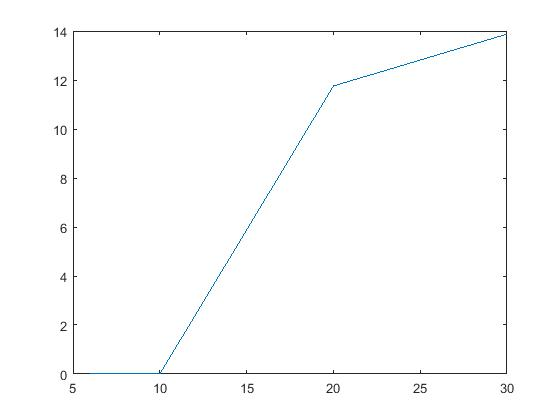
\includegraphics[width=9cm]{grafo1-rfe}
 				\caption{Gráfico del error relativo $rfe$}	
 			\end{figure}
 			
 			\begin{figure}[H]
 				\centering
 				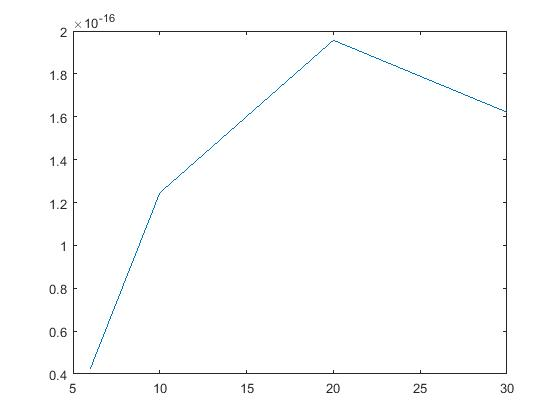
\includegraphics[width=9cm]{grafo1-rbe}
 				\caption{Gráfico del error relativo $rfb$}		
 			\end{figure}
 			
 			\begin{figure}[H]
 				\centering
 				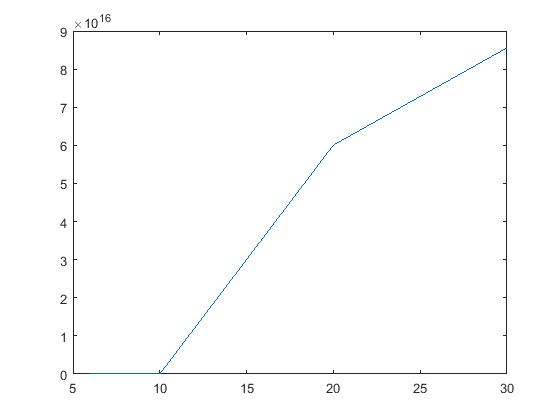
\includegraphics[width=9cm]{grafo1-div}
 				\caption{Gráfico de$\frac{rfe}{rbe}$}
	
 			\end{figure}
 		
 			En el primer gráfico se puede observar que para matrices de menor tamaño, el error es despreciable, pero a medida que el tamaño de la matriz aumenta también lo hace su error. Esto se produce debido al mal condicionamiento de la matriz de Hilbert.
 		\end{enumerate}
 		
 	Para resolver este problema se ocuparon los siguientes archivos: SolLU.m, FactorizacionLU.m, DiagUp.m y DiagDown.m	
 	\newpage
 	\item 
 	 \begin{enumerate}
 	    \item Usando la Factorización de Cholesky, encuentre la solución del sistema $A^{T}Ax = b$, con $b \in R^{n}$  un vector de unos, cuando n = 10, 20, 30.
 	        \begin{align*}
 	             1) \left(\begin{array}{c} 0.7347\\ 0.8712\\ 0.9332\\ 1.0677\\ 1.0839\\ 1.0830\\ 1.0269\\ 0.8574\\ 0.8229\\ 0.6498 \end{array}\right) 	 &&   2) \left(\begin{array}{c} 0.8160\\ 0.9860\\ 1.0786\\ 1.2779\\ 1.3690\\ 1.4156\\ 1.4739\\ 1.5073\\ 1.5207\\ 1.5299\\ 1.5233\\ 1.5040\\ 1.4823\\ 1.4311\\ 1.3565\\ 1.3074\\ 1.1858\\ 0.9651\\ 0.9069\\ 0.7025 \end{array}\right)   &&  3) \left(\begin{array}{c} 0.8227\\ 0.9954\\ 1.0912\\ 1.2954\\ 1.3919\\ 1.4450\\ 1.5117\\ 1.5567\\ 1.5841\\ 1.6098\\ 1.6289\\ 1.6408\\ 1.6496\\ 1.6550\\ 1.6563\\ 1.6548\\ 1.6503\\ 1.6411\\ 1.6285\\ 1.6125\\ 1.5863\\ 1.5536\\ 1.5207\\ 1.4604\\ 1.3791\\ 1.3247\\ 1.1986\\ 0.9740\\ 0.9136\\ 0.7067 \end{array}\right) 
 	        \end{align*}
	        
 	        \item Para n = 10 hasta n = 60, cálcule el número condición de la matriz A (use la norma $\norm{.}_{\infty}$). Represente en una gráfica el resultado obtenido (n vs. cond(A)). Que puede decir de la matriz A.\\
 	        
 	        La gráfica obtenida fue la siguiente :
            \begin{figure}[H]
                \centering
                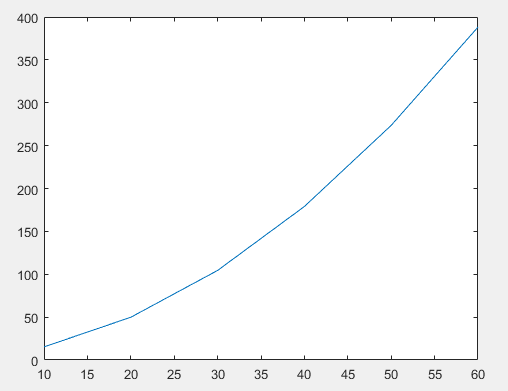
\includegraphics[width=8cm]{Grafico2b}
                \caption{Gráfico n vs K(A)} \label{fig:Grafico2b}
            \end{figure}
       \end{enumerate}     
            Gracias a el resultado obtenido se puede apreciar claramente un aumento casi cuadrático del mal comportamiento de la matriz a mientras incrementa su orden matricial.Esto quiere decir que a medida que aumenta el tamaño de la matriz el determinante tiende a cero rapidamente.\\
            
             	Para resolver este problema se ocuparon los siguientes archivos: SolLU.m, FactorizacionLU.m, DiagUp.m, DiagDown.m,Diag.m,Matrix2.m,Sol\_problema2.m,NumCondicion.m y NormInf.m	
        \item
        \item
                \begin{enumerate}
            \item Suponiendo que m = n, encuentre la solución del sistema anterior vía eliminación Gaussiana, cuando n = 8,15,20,50.
            \begin{table}[H]
        \centering
            \begin{tabular} {|c|}
            \hline
            Valores de la solución para n=8 \\
            \hline
            x_{1}=  0,42005\\
            \hline
            x_{2}=  -1,86380\\
            \hline
            x_{3}=  0,06716\\
            \hline
            x_{4}=  8,71470\\
            \hline
            x_{5}=  -2,26160\\
            \hline
            x_{6}=  -13,872\\
            \hline
            x_{7}=  1,82990\\
            \hline
            x_{8}=  7,0035\\
            \hline
            \end{tabular}
        \end{table}
        
        \begin{table}[H]
        \centering
            \begin{tabular} { |c|}
            
            \hline
            Valores de la solución para n=15 \\
            \hline
            x_{1}= 0,66216\\
            \hline
            x_{2}=  -3,2558\\
            \hline
            x_{3}=  2,5351\\
            \hline
            x_{4}=  51,084\\
            \hline
            x_{5}=  -142,67\\
            \hline
            x_{6}=  -349,97\\
            \hline
            x_{7}=  1267,5\\
            \hline
            x_{8}=  1219,3\\
            \hline
            x_{9}=  -4939\\
            \hline
            x_{10}= -2212,5\\
            \hline
            x_{11}= 9501,1\\
            \hline
            x_{12}= 1972,1\\
            \hline
            x_{13}= -8758,3\\
            \hline
            x_{14}= -676,7\\
            \hline
            x_{15}= 3068,2\\
            \hline
            \end{tabular}
        \end{table}
        
        \begin{table}[H]
        \centering
            \begin{tabular} {|c|}
            
            \hline
            Valores de la solución para n=20 \\
            \hline
            x_{1}= 0,78893\\
            \hline
            x_{2}=  -3,242\\
            \hline
            x_{3}=  -4,634\\
            \hline
            x_{4}=  78,394\\
            \hline
            x_{5}=  -62,354\\
            \hline
            x_{6}=  -999,57\\
            \hline
            x_{7}=  1236,5\\
            \hline
            x_{8}=  7758,6\\
            \hline
            x_{9}=  -8888,8\\
            \hline
            x_{10}= -37882\\
            \hline
            x_{11}= 34023\\
            \hline
            x_{12}= 1,17E+05\\
            \hline
            x_{13}= -74840\\
            \hline
            x_{14}= -2,25E+05\\
            \hline
            x_{15}= 94271\\
            \hline
            x_{16}= 2,60E+05\\
            \hline
            x_{17}= -62902\\
            \hline
            x_{18}= -1,64E+05\\
            \hline
            x_{19}= 17167\\
            \hline
            x_{20}= 42838\\
            \hline
            \end{tabular}
        \end{table}

\centering  
\begin{tabular}{ |l|l| }
  \hline
  \multicolumn{2}{|c|}{Valores de la solución para n=50 } \\
  \hline
   x_{1}= 0,95399 & x_{26}= 1,16E+09\\
x_{2}= -2,0286 & x_{27}= 1,10E+09\\
x_{3}= -20,884 & x_{28}= -4,92E+08\\
x_{4}= 80,9 & x_{29}= -1,05E+09\\
x_{5}= 429,77 & x_{30}= 2,60E+08\\
x_{6}= -1853,9 & x_{31}= 5,09E+08\\
x_{7}= -7667,8 & x_{32}= -4,34E+08\\
x_{8}= 27248 & x_{33}= -2,05E+08\\
x_{9}= 1,04E+05 & x_{34}= 3,96E+08\\
x_{10}= -2,85E+05 & x_{35}= 2,03E+08\\
x_{11}= -1,09E+06 & x_{36}= -1,38E+08\\
x_{12}= 2,08E+06 & x_{37}= -5,73E+07\\
x_{13}= 8,92E+06 & x_{38}= 1,22E+08\\
x_{14}= -8,88E+06 & x_{39}= -1,72E+08\\
x_{15}= -5,28E+07 & x_{40}= -1,89E+08\\
x_{16}= 1,16E+07 & x_{41}= 1,51E+08\\
x_{17}= 2,09E+08 & x_{42}= 8,63E+06\\
x_{18}= 7,42E+07 & x_{43}= 5,75E+06\\
x_{19}= -5,27E+08 & x_{44}= 1,35E+08\\
x_{20}= -4,32E+08 & x_{45}= -8,43E+07\\
x_{21}= 7,91E+08 & x_{46}= -7,38E+07\\
x_{22}= 1,07E+09 & x_{47}= 7,20E+07\\
x_{23}= -5,20E+08 & x_{48}= 1,16E+07\\
x_{24}= -1,48E+09 & x_{49}= -2,34E+07\\
x_{25}= -3,58E+08 & $x_{50} = -2,30E+06$\\
\hline
\end{tabular}
\newpage
\item Grafique la función $f$ versus el polinomio $g$ para $n = 8$, $15$, $20$, $50$. Comente sus resultados.
    \begin{figure}[H]
    \centering
    \subfloat[$n=8$]{{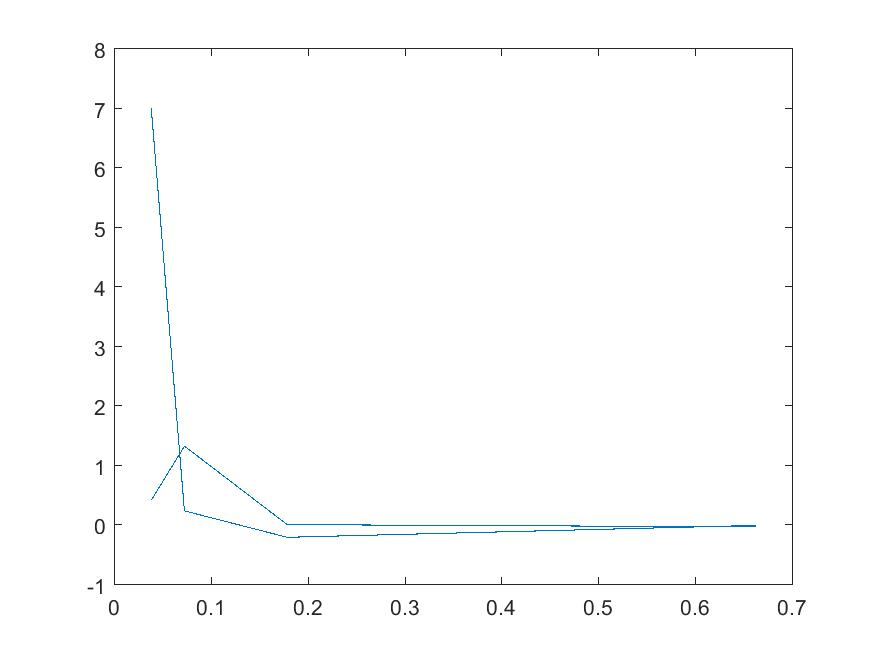
\includegraphics[width=9cm]{datos-8}}}
    \subfloat[$n=15$]{{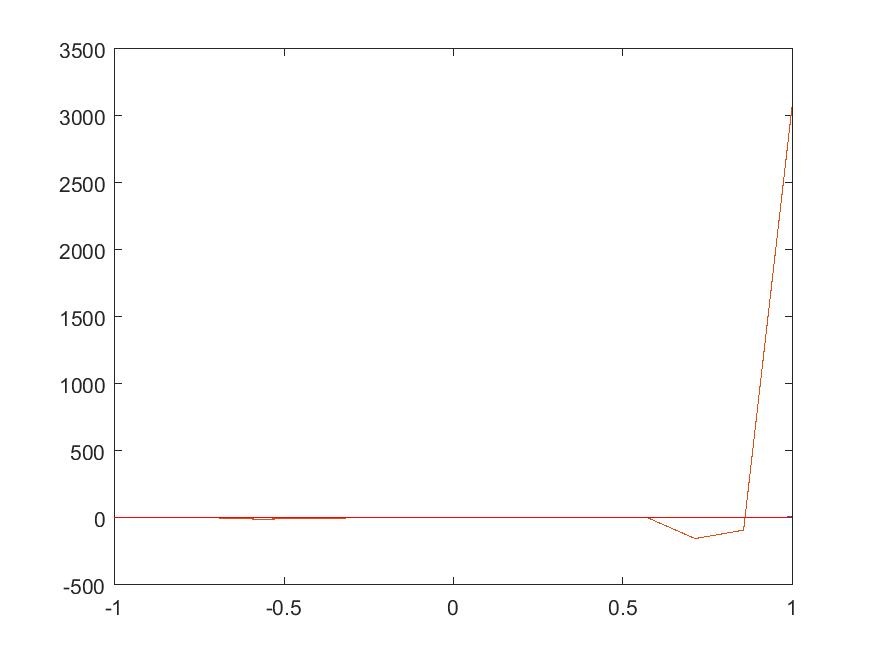
\includegraphics[width=9cm]{datos-15} }}
    \hfill
    \subfloat[$n=20$]{{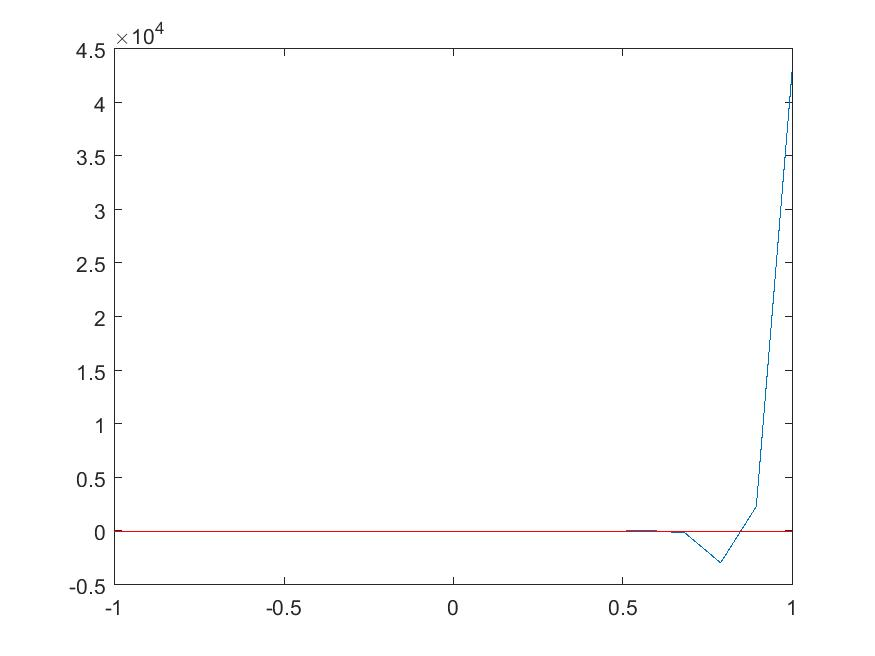
\includegraphics[width=9cm]{datos-20} }}
    \subfloat[$n=50$]{{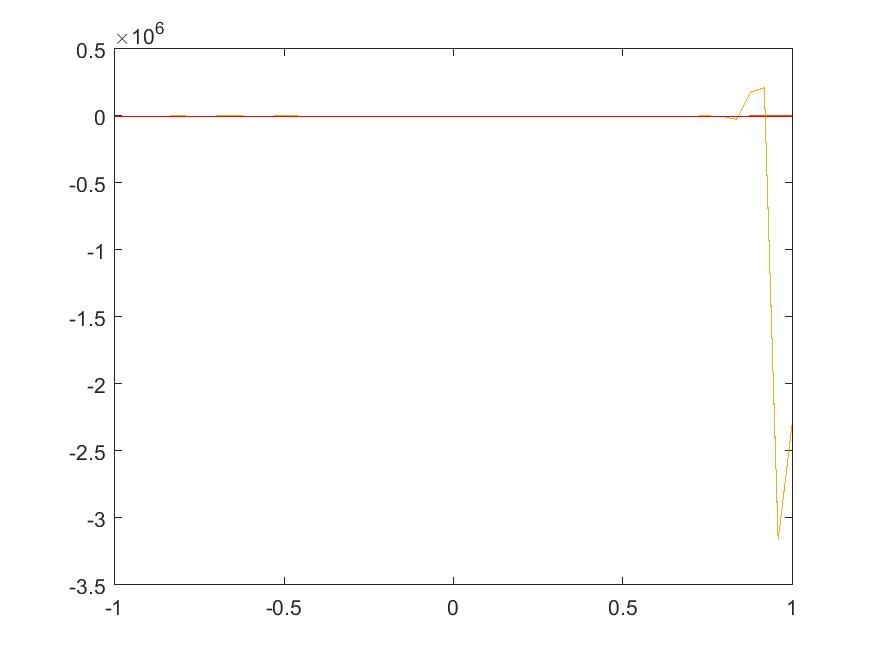
\includegraphics[width=9cm]{datos-50} }}
    \end{figure}
     
Los gráficos debiesen ser iguales, pero la gráfica del polinomio $g$ se dispara a valores muy altos cuando $t>0,5$

     \end{enumerate}
       %%%%%%%%%%%%%%%
 %pregunta 5
 %%%%%%%%%%%%%%%%	
 	\item 
 	\begin{enumerate}
 			\item \begin{itemize}
 				\item Al ocupar el método de Richardson, en ambos casos, la matriz definida por $I-M^5$ tiene un radio espectral mayor a 1. Siendo 1.0084 cuando $n=20$ y 1.0091 para $n=40$
 				\item Lo mismo sucede con el método de Jacobi. Cuando $n = 20$, el radio espectral de la matriz definida por $I-Q^{-1}M^5$ tiene un valor de 3.8417, mientras que vale 3.8517 cuando  $n=40$.
 				\item Al ocupar el método de Gauss-Seidel, se encuentre el mismo inconveniente. Con valores del radio espectral 1.0862 y 1.0945, respectivamente.
 				\item Por último, cuando se uitliza el método de Relajación, nuevamente, se encuentra el mismo problema. Esta vez, los valores del radio espectral cuando $n=20$ son 1.0222, 1.0338 y 1.0382, para $w=0.7, 1.3,1.6$ respectivamente. Pr otra parte, cuando $n=40$, este vale 1.0242, 1.0369, 1.0432 para los respectivos valores de $w$
 			\end{itemize}
 			\newpage
 			\item Para todos los métodos se ocupó una tolerancia de 0.0001 y como criterio de parada se utilizó $\frac{\norm{x^{k+1}-x^{k}}_{2}}{\norm{x^{k+1}}_{2}}\leq 0.0001$. 
 			Como ninguno de los métodos convergió, no se puede calcular la cantidad de iteraciones ni el tiempo utilizado.
 			
		\end{enumerate} 	  
 %%%%%%%%%%%%%%%
 %pregunta 6
 %%%%%%%%%%%%%%%%	
	\item
 		\begin{enumerate}
			\item Como la matriz de coeficientes no tiene filas nulas ni filas que sean multiplos de otras, se puede afirmar que el determinante siempre es distinto de 0. Esto nos demuestra que esta matriz tiene una solución única. Para demostrar que el vector $x_{e} = \frac{1}{n+1}(1,2,...,n)$ es solución del sistema, ocuparemos una matriz de $6 \times 6$ a modo de ejemplo.
			\begin{equation}
				\textrm{El sistema definido por} Ax = b
				\textrm{ Donde } A = \left(\begin{array}{cccccc} 2.0 & -1.0 & 0 & 0 & 0 & 0\\ -1.0 & 2.0 & -1.0 & 0 & 0 & 0\\ 0 & -1.0 & 2.0 & -1.0 & 0 & 0\\ 0 & 0 & -1.0 & 2.0 & -1.0 & 0\\ 0 & 0 & 0 & -1.0 & 2.0 & -1.0\\ 0 & 0 & 0 & 0 & -1.0 & 2.0 \end{array}\right)
				\textrm{ y } x_{e} = \left(\begin{array}{c} 0.1667\\ 0.3333\\ 0.5\\ 0.6667\\ 0.8333\\ 1.0 \end{array}\right)
			\end{equation}			 
			
			Luego 
			\begin{equation}
				b = Ax_{e}
			\end{equation}
			
			Entonces el vector b tiene un valor de $\left(\begin{array}{c} 0\\ 0\\ 1.11\cdot 10^{-16}\\ 0\\ -1.11\cdot 10^{-16}\\ 1.167 \end{array}\right)$
			Luego si calculamos el error relativo entre este vector $b$ y el vector $b$ real, definido por $\frac{\norm{b_{e}-b}}{\norm{b_{e}}}$ donde $b_{e}$ sería este último, obtenemos un valor de 0.1667. 
			
			Por lo tanto, se concluye que el vector $x_{e} = \frac{1}{n+1}$
			
			\item 	
			\begin{itemize}
				\item Cuando se ocupa el método de Richardson, este no converge para ninguno de los tres casos, ya que los valores del radio espectral de la matriz definida por $I-A$ son mayores a 1. Teniendo valores de 2.9854, 2.9962, 2.9973 para $n=25, n=50$ y $n=60$ respectivamente.
				
				\item Al ocupar el método de Jacobi con una tolerancia de 0.0001, se obtienen los siguientes valores para:
				
					 n = 25: 
					$x_{a} = \left(\begin{array}{c} 0.03939\\ 0.07875\\ 0.1181\\ 0.1574\\ 0.1967\\ 0.2358\\ 0.275\\ 0.314\\ 0.353\\ 0.3917\\ 0.4305\\ 0.4691\\ 0.5077\\ 0.546\\ 0.5844\\ 0.6225\\ 0.6606\\ 0.6986\\ 0.7365\\ 0.7743\\ 0.8121\\ 0.8497\\ 0.8873\\ 0.9249\\ 0.9625 \end{array}\right) $	
					 n = 50:
					$x_{a} = \left(\begin{array}{c} 0.0215\\ 0.04301\\ 0.06448\\ 0.08595\\ 0.1074\\ 0.1288\\ 0.1501\\ 0.1715\\ 0.1927\\ 0.2139\\ 0.235\\ 0.2561\\ 0.277\\ 0.2979\\ 0.3187\\ 0.3394\\ 0.36\\ 0.3805\\ 0.4009\\ 0.4212\\ 0.4414\\ 0.4615\\ 0.4814\\ 0.5013\\ 0.521\\ 0.5406\\ 0.5601\\ 0.5795\\ 0.5987\\ 0.6179\\ 0.6369\\ 0.6558\\ 0.6746\\ 0.6934\\ 0.7119\\ 0.7305\\ 0.7489\\ 0.7672\\ 0.7854\\ 0.8036\\ 0.8217\\ 0.8398\\ 0.8577\\ 0.8756\\ 0.8935\\ 0.9113\\ 0.9291\\ 0.9468\\ 0.9646\\ 0.9823 \end{array}\right)$
										
					 n = 60:	
					$x_{a} = \left(\begin{array}{c} 0.0187\\ 0.03739\\ 0.05608\\ 0.07474\\ 0.09339\\ 0.112\\ 0.1306\\ 0.1491\\ 0.1676\\ 0.186\\ 0.2044\\ 0.2227\\ 0.2409\\ 0.2591\\ 0.2772\\ 0.2952\\ 0.3131\\ 0.3309\\ 0.3487\\ 0.3663\\ 0.3838\\ 0.4012\\ 0.4186\\ 0.4357\\ 0.4529\\ 0.4698\\ 0.4867\\ 0.5034\\ 0.5201\\ 0.5366\\ 0.553\\ 0.5692\\ 0.5854\\ 0.6014\\ 0.6174\\ 0.6332\\ 0.6489\\ 0.6644\\ 0.6799\\ 0.6953\\ 0.7106\\ 0.7257\\ 0.7408\\ 0.7557\\ 0.7706\\ 0.7853\\ 0.8001\\ 0.8147\\ 0.8293\\ 0.8437\\ 0.8581\\ 0.8725\\ 0.8868\\ 0.901\\ 0.9153\\ 0.9294\\ 0.9436\\ 0.9577\\ 0.9718\\ 0.9859 \end{array}\right)$
			
				\item Cuando se utiliza el método de Gauss-Seidel con la misma tolerancia, los resultados son los siguientes:
				
				n = 25:
				$x_{a} = \left(\begin{array}{c} 0.03939\\ 0.07875\\ 0.1181\\ 0.1574\\ 0.1967\\ 0.2358\\ 0.275\\ 0.314\\ 0.353\\ 0.3917\\ 0.4305\\ 0.4691\\ 0.5077\\ 0.546\\ 0.5844\\ 0.6225\\ 0.6606\\ 0.6986\\ 0.7365\\ 0.7743\\ 0.8121\\ 0.8497\\ 0.8873\\ 0.9249\\ 0.9625 \end{array}\right)$
				n = 50:
				$x_{a} = \left(\begin{array}{c} 0.021\\ 0.04198\\ 0.06295\\ 0.0839\\ 0.1048\\ 0.1257\\ 0.1466\\ 0.1674\\ 0.1882\\ 0.2089\\ 0.2296\\ 0.2502\\ 0.2707\\ 0.2912\\ 0.3116\\ 0.332\\ 0.3523\\ 0.3725\\ 0.3926\\ 0.4127\\ 0.4326\\ 0.4525\\ 0.4723\\ 0.4921\\ 0.5117\\ 0.5313\\ 0.5508\\ 0.5702\\ 0.5895\\ 0.6088\\ 0.6279\\ 0.647\\ 0.6661\\ 0.685\\ 0.7039\\ 0.7227\\ 0.7415\\ 0.7602\\ 0.7788\\ 0.7974\\ 0.816\\ 0.8345\\ 0.853\\ 0.8714\\ 0.8898\\ 0.9082\\ 0.9266\\ 0.945\\ 0.9633\\ 0.9817 \end{array}\right)$
				
				
				n = 60:
				$x_{a} = \left(\begin{array}{c} 0.0187\\ 0.03739\\ 0.05608\\ 0.07474\\ 0.09339\\ 0.112\\ 0.1306\\ 0.1491\\ 0.1676\\ 0.186\\ 0.2044\\ 0.2227\\ 0.2409\\ 0.2591\\ 0.2772\\ 0.2952\\ 0.3131\\ 0.3309\\ 0.3487\\ 0.3663\\ 0.3838\\ 0.4012\\ 0.4186\\ 0.4357\\ 0.4529\\ 0.4698\\ 0.4867\\ 0.5034\\ 0.5201\\ 0.5366\\ 0.553\\ 0.5692\\ 0.5854\\ 0.6014\\ 0.6174\\ 0.6332\\ 0.6489\\ 0.6644\\ 0.6799\\ 0.6953\\ 0.7106\\ 0.7257\\ 0.7408\\ 0.7557\\ 0.7706\\ 0.7853\\ 0.8001\\ 0.8147\\ 0.8293\\ 0.8437\\ 0.8581\\ 0.8725\\ 0.8868\\ 0.901\\ 0.9153\\ 0.9294\\ 0.9436\\ 0.9577\\ 0.9718\\ 0.9859 \end{array}\right)$
				\item Finalmente,al utilizar el método de Relajación, se se encuentran las siguientes soluciones, dependiendo del valor de $w$:
				\begin{itemize}
				\item $w = 0.5$:
				n = 25: $x_{a} = \left(\begin{array}{c} 0.04188\\ 0.08371\\ 0.1254\\ 0.167\\ 0.2083\\ 0.2495\\ 0.2903\\ 0.3308\\ 0.371\\ 0.4108\\ 0.4502\\ 0.4893\\ 0.5279\\ 0.5661\\ 0.6039\\ 0.6413\\ 0.6784\\ 0.7151\\ 0.7515\\ 0.7875\\ 0.8233\\ 0.8589\\ 0.8944\\ 0.9296\\ 0.9648 \end{array}\right)$ 
				n = 50: $x_{a} = \left(\begin{array}{c} 0.02703\\ 0.05402\\ 0.08095\\ 0.1078\\ 0.1345\\ 0.1611\\ 0.1875\\ 0.2137\\ 0.2397\\ 0.2654\\ 0.2908\\ 0.316\\ 0.3409\\ 0.3654\\ 0.3895\\ 0.4133\\ 0.4367\\ 0.4597\\ 0.4823\\ 0.5045\\ 0.5263\\ 0.5476\\ 0.5684\\ 0.5888\\ 0.6088\\ 0.6283\\ 0.6474\\ 0.666\\ 0.6842\\ 0.7019\\ 0.7192\\ 0.7361\\ 0.7526\\ 0.7687\\ 0.7845\\ 0.7998\\ 0.8148\\ 0.8295\\ 0.8438\\ 0.8579\\ 0.8717\\ 0.8852\\ 0.8986\\ 0.9117\\ 0.9246\\ 0.9374\\ 0.9501\\ 0.9627\\ 0.9751\\ 0.9876 \end{array}\right)$	
				
				n = 60: $x_{a} = \left(\begin{array}{c} 0.02591\\ 0.0518\\ 0.07762\\ 0.1034\\ 0.129\\ 0.1545\\ 0.1798\\ 0.2049\\ 0.2299\\ 0.2545\\ 0.279\\ 0.3031\\ 0.327\\ 0.3505\\ 0.3737\\ 0.3965\\ 0.4189\\ 0.441\\ 0.4627\\ 0.4839\\ 0.5047\\ 0.5251\\ 0.545\\ 0.5644\\ 0.5834\\ 0.6019\\ 0.62\\ 0.6376\\ 0.6546\\ 0.6713\\ 0.6874\\ 0.7031\\ 0.7183\\ 0.733\\ 0.7473\\ 0.7611\\ 0.7745\\ 0.7874\\ 0.7999\\ 0.812\\ 0.8237\\ 0.8351\\ 0.846\\ 0.8566\\ 0.8669\\ 0.8768\\ 0.8864\\ 0.8958\\ 0.9049\\ 0.9137\\ 0.9223\\ 0.9306\\ 0.9388\\ 0.9468\\ 0.9547\\ 0.9624\\ 0.9701\\ 0.9776\\ 0.9851\\ 0.9926 \end{array}\right)$	
				
				\item $w = 1.2$:
				n = 25: $x_{a} = \left(\begin{array}{c} 0.04028\\ 0.08052\\ 0.1207\\ 0.1608\\ 0.2008\\ 0.2406\\ 0.2803\\ 0.3199\\ 0.3592\\ 0.3984\\ 0.4373\\ 0.4761\\ 0.5146\\ 0.5529\\ 0.591\\ 0.6289\\ 0.6666\\ 0.7042\\ 0.7415\\ 0.7787\\ 0.8158\\ 0.8528\\ 0.8896\\ 0.9265\\ 0.9632 \end{array}\right)$
				n = 50: $x_{a} = \left(\begin{array}{c} 0.02336\\ 0.0467\\ 0.07\\ 0.09326\\ 0.1165\\ 0.1396\\ 0.1626\\ 0.1855\\ 0.2083\\ 0.231\\ 0.2536\\ 0.276\\ 0.2982\\ 0.3203\\ 0.3422\\ 0.3639\\ 0.3855\\ 0.4068\\ 0.4279\\ 0.4488\\ 0.4695\\ 0.49\\ 0.5102\\ 0.5302\\ 0.55\\ 0.5696\\ 0.5889\\ 0.608\\ 0.6269\\ 0.6456\\ 0.664\\ 0.6823\\ 0.7003\\ 0.7181\\ 0.7358\\ 0.7532\\ 0.7705\\ 0.7876\\ 0.8046\\ 0.8214\\ 0.8381\\ 0.8546\\ 0.8711\\ 0.8874\\ 0.9036\\ 0.9198\\ 0.9359\\ 0.952\\ 0.968\\ 0.984 \end{array}\right)$
				
				n = 60: $x_{a} = \left(\begin{array}{c} 0.02101\\ 0.04201\\ 0.06297\\ 0.0839\\ 0.1048\\ 0.1256\\ 0.1463\\ 0.1669\\ 0.1875\\ 0.2079\\ 0.2282\\ 0.2484\\ 0.2684\\ 0.2883\\ 0.308\\ 0.3276\\ 0.347\\ 0.3662\\ 0.3852\\ 0.404\\ 0.4225\\ 0.4409\\ 0.4591\\ 0.4771\\ 0.4948\\ 0.5123\\ 0.5295\\ 0.5466\\ 0.5634\\ 0.58\\ 0.5963\\ 0.6124\\ 0.6283\\ 0.6439\\ 0.6593\\ 0.6745\\ 0.6895\\ 0.7042\\ 0.7188\\ 0.7331\\ 0.7472\\ 0.7611\\ 0.7749\\ 0.7884\\ 0.8018\\ 0.815\\ 0.8281\\ 0.841\\ 0.8538\\ 0.8664\\ 0.879\\ 0.8914\\ 0.9037\\ 0.9159\\ 0.9281\\ 0.9401\\ 0.9522\\ 0.9642\\ 0.9761\\ 0.9881 \end{array}\right)$
				
				\item $w = 1.65$:	
				n = 25: $x_{a} = \left(\begin{array}{c} 0.03998\\ 0.07992\\ 0.1198\\ 0.1596\\ 0.1993\\ 0.239\\ 0.2784\\ 0.3178\\ 0.357\\ 0.396\\ 0.4349\\ 0.4736\\ 0.5121\\ 0.5504\\ 0.5886\\ 0.6266\\ 0.6644\\ 0.7021\\ 0.7396\\ 0.7771\\ 0.8144\\ 0.8516\\ 0.8888\\ 0.9259\\ 0.9629 \end{array}\right)$
				n = 50: $x_{a} = \left(\begin{array}{c} 0.02269\\ 0.04537\\ 0.06802\\ 0.09063\\ 0.1132\\ 0.1357\\ 0.1581\\ 0.1804\\ 0.2027\\ 0.2248\\ 0.2468\\ 0.2687\\ 0.2905\\ 0.3122\\ 0.3336\\ 0.355\\ 0.3761\\ 0.3972\\ 0.418\\ 0.4387\\ 0.4591\\ 0.4795\\ 0.4996\\ 0.5195\\ 0.5393\\ 0.5588\\ 0.5782\\ 0.5974\\ 0.6164\\ 0.6352\\ 0.6539\\ 0.6724\\ 0.6907\\ 0.7088\\ 0.7268\\ 0.7447\\ 0.7624\\ 0.7799\\ 0.7974\\ 0.8147\\ 0.8319\\ 0.849\\ 0.866\\ 0.8829\\ 0.8998\\ 0.9166\\ 0.9333\\ 0.95\\ 0.9667\\ 0.9833 \end{array}\right)$
				
				n = 60: $x_{a} =\left(\begin{array}{c} 0.02017\\ 0.04033\\ 0.06046\\ 0.08056\\ 0.1006\\ 0.1206\\ 0.1406\\ 0.1604\\ 0.1802\\ 0.1999\\ 0.2195\\ 0.239\\ 0.2583\\ 0.2776\\ 0.2967\\ 0.3157\\ 0.3345\\ 0.3532\\ 0.3717\\ 0.39\\ 0.4082\\ 0.4262\\ 0.4441\\ 0.4617\\ 0.4792\\ 0.4965\\ 0.5136\\ 0.5305\\ 0.5473\\ 0.5638\\ 0.5802\\ 0.5963\\ 0.6123\\ 0.628\\ 0.6436\\ 0.659\\ 0.6743\\ 0.6893\\ 0.7042\\ 0.7189\\ 0.7334\\ 0.7478\\ 0.762\\ 0.7761\\ 0.79\\ 0.8038\\ 0.8175\\ 0.8311\\ 0.8445\\ 0.8578\\ 0.8711\\ 0.8842\\ 0.8973\\ 0.9103\\ 0.9232\\ 0.9361\\ 0.9489\\ 0.9617\\ 0.9745\\ 0.9872 \end{array}\right)$
				\end{itemize}
			\end{itemize}
			\item Para todos los métodos se ocupó una tolerancia de 0.0001 y como criterio de parada se utilizó $\frac{\norm{x^{k+1}-x^{k}}_{2}}{\norm{x^{k+1}}_{2}}\leq 0.0001$. 
			\begin{itemize}
				\item Jacobi:
					\begin{table}[H]
						\centering
						\begin{tabular}{|c|c|c|c|c|}
							\hline 
							n & Iteraciones & Tiempo (s) & Convergencia & Error \\
							\hline
							25 & 603 &0.2313 & 0.9927 & 0.0080 \\
							\hline
							50 & 1594 & 0.8390 & 0.9927 & 0.0314 \\
							\hline
							60 & 19999 & 1.1572 & 0.9987 & 0.0456 \\
							\hline
						\end{tabular}
					\end{table}
				\item Gauss-Seidel:
				 \begin{table}[H]
						\centering
						\begin{tabular}{|c|c|c|c|c|}
							\hline 
							n & Iteraciones & Tiempo & Convergencia & Error \\
							\hline
							25 &603 & 0.0339 & 0.9855 & 0.008 \\
							\hline
							50 & 1594 & 0.0716 & 0.9962 & 0.0314 \\
							\hline
							60 & 19999 & 0.1228 & 0.9973 & 0.0456 \\
							\hline
						\end{tabular}
					\end{table}
				\item Relajación:
					\begin{itemize}
					\item $w=0.5$
						\begin{table}[H]
						\centering
						\begin{tabular}{|c|c|c|c|c|}
							\hline 
							n & Iteraciones & Tiempo & Convergencia & Error \\
							\hline
							25 & 1065 & 0.0154 & 0.9971 & 0.0290 \\
							\hline
							50 & 2021 & 0.1959 & 0.9992 & 0.1210 \\
							\hline
							60 & 2372 & 0.0204 & 0.9995 & 0.1824\\
							\hline
						\end{tabular}
					\end{table}
					\item $w=1.2$
					\begin{table}[H]
						\centering
						\begin{tabular}{|c|c|c|c|c|}
							\hline 
							n & Iteraciones & Tiempo & Convergencia & Error \\
							\hline
							25 & 683 & 0.0126 & 0.9943 & 0.0152\\
							\hline
							50 & 1649 & 0.0251 & 0.9986 & 0.0610 \\
							\hline
							60 & 1972 & 0.0196 & 0.9990 & 0.0896  \\
							\hline
						\end{tabular}
					\end{table}
					\item $w=1.65$
					\begin{table}[H]
						\centering
						\begin{tabular}{|c|c|c|c|c|}
							\hline 
							n & Iteraciones & Tiempo & Convergencia & Error \\
							\hline
							25 & 594 & 0.0123 & 0.9934 & 0.0126 \\
							\hline
							50 & 1481 & 0.0176 & 0.9983 & 0.0500 \\
							\hline
							60 & 1802 & 0.0180 & 0.9988 & 0.0732 \\
							\hline
						\end{tabular}
					\end{table}
					\end{itemize}			
			\end{itemize}
 	        Se puede observar que la cantidad de iteraciones y el error de los métodos de Gauss-Seidel y Jacobi tienen los mismos valores, aunque este último toma más tiempo.
 	        \\
			Por otra, parte al analizar los resultados del método de Relajación para los diferentes valores de $w$, se puede percatar de que a entre más grande es el valor de $w$, más rápido converge, además de que disminuye el error. \newpage
 	        \item Los resultados encontrados al utilizar la forma general del método de Gauss-Seidel, son:
 	        
 	        n = 25: 
 	       	$x_{a} = \left(\begin{array}{c} 0.03916\\ 0.0783\\ 0.1174\\ 0.1565\\ 0.1955\\ 0.2345\\ 0.2734\\ 0.3122\\ 0.351\\ 0.3897\\ 0.4283\\ 0.4669\\ 0.5053\\ 0.5437\\ 0.582\\ 0.6203\\ 0.6584\\ 0.6965\\ 0.7346\\ 0.7726\\ 0.8105\\ 0.8485\\ 0.8864\\ 0.9243\\ 0.9621 \end{array}\right) $
 	        n = 50:
 	        $x_{a} = \left(\begin{array}{c} 0.03916\\ 0.0783\\ 0.1174\\ 0.1565\\ 0.1955\\ 0.2345\\ 0.2734\\ 0.3122\\ 0.351\\ 0.3897\\ 0.4283\\ 0.4669\\ 0.5053\\ 0.5437\\ 0.582\\ 0.6203\\ 0.6584\\ 0.6965\\ 0.7346\\ 0.7726\\ 0.8105\\ 0.8485\\ 0.8864\\ 0.9243\\ 0.9621 \end{array}\right)$
 	        
 	        Con esta información se pueden armar las siguientes tabla comparativas:
 	        \begin{itemize}
 	        	\item Para n=25: \begin{table}[H]
 	        			\centering
 	        			\begin{tabular}{|c|c|c|}
 	        				\hline 
							 & General & Implementable \\
							 \hline
							 Tiempo & 0.0183 & 0.0339 \\
							 \hline
							 Iteraciones & 320 & 603\\
							 \hline
							 Error & 0.0055 & 0.0080\\
							\hline
 	        			\end{tabular}
 	        		\end{table}
 	        		\item Para n=50: \begin{table}[H]
 	        			\centering
 	        			\begin{tabular}{|c|c|c|}
 	        				\hline 
							 & General & Implementable \\
							 \hline
							 Tiempo & 0.0167 & 0.0716 \\
							 \hline
							 Iteraciones & 879 & 1594 \\
							 \hline
							 Error & 0.0220 & 0.0314\\
							\hline
 	        			\end{tabular}
 	        		\end{table}
 	        		Con estos datos, se puede concluír que la forma general del método de Gauss-Seidel es mucho más efectiva a la hora de resolver un sistema que su contraparte implementable. Esto debido a que en ambos casos, la forma general presenta un menor tiempo de ejecución, una menor cantidad de iteracionas y un menor error.
 	        		\\
 	        		Para responder esta pregunta se utilizaron los archivos GaussSeidel.m, Jacobi2.m, gs-implementable.m y Richardson.m
 	        \end{itemize}
 	 \end{enumerate}
 \end{enumerate}
 

\newpage
\chapter{Aproximación de funciones} 
\begin{enumerate}
    
\vspace{0.9cm}
\item 

Se desea dibujar el contorno del auto de la siguiente foto:

\begin{figure}[H]
    \centering
    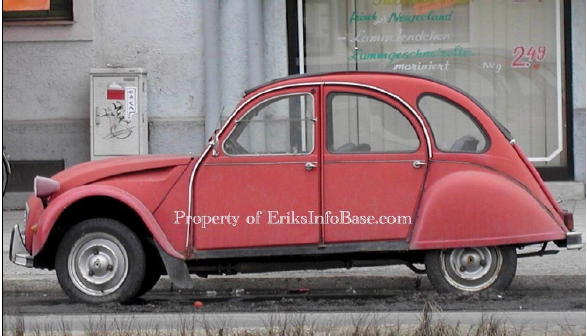
\includegraphics[width=10cm]{enun1}
    \caption{enunciado.} \label{fig:enun1}
\end{figure}


Basado en esta figura se han obtenido los siguientes puntos:



\begin{table}[H]
    \centering
        \begin{tabular} { |c|c|}
        
        \hline
        xi  &  yi\\
        \hline
        2 &  5       \\
         \hline
        2.7 &  7.8        \\
         \hline
        3.8 &  9        \\
         \hline
        7 &  10        \\
         \hline
        8 &  10.2        \\
         \hline
        10 & 10.3        \\
         \hline
        13 & 10.4          \\
         \hline
        16 &  14.5        \\
         \hline
        18 &  15       \\
         \hline
        21 &  15.4        \\
         \hline
        25 &  15.5       \\
         \hline
        30 &  14       \\
        \hline
        36& 5   \\
        \hline
        \end{tabular}
        \caption{Puntos superiores.}
    \end{table}
 \vspace{1.8cm}
 
 \begin{table}[H]
    \centering
        \begin{tabular} { |c|c|}
        
        \hline
        xi  &  yi\\
        \hline
        2 &  5       \\
         \hline
        3 &  4        \\
         \hline
        7 &  7.9        \\
         \hline
        12 &  3.8        \\
         \hline
        22 &  4        \\
         \hline
        29 & 4.6        \\
        \hline
        \end{tabular}
        \caption{Puntos inferiores.}
    \end{table}
 \begin{itemize}
\item Utilizando la interpolación por Spline cubico, obtenga las dos curvas que aproximan el contorno del auto.
\end{itemize}

\begin{figure}[H]
    \centering
    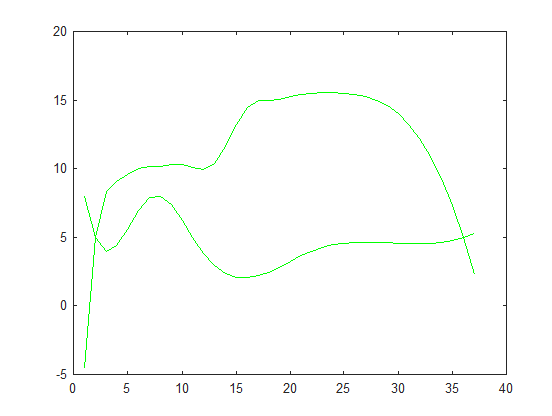
\includegraphics[width=9cm]{interp_spline}
    \caption{interpolación Spline cubica.} \label{fig:interp_spline}
\end{figure}

\begin{figure}[H]
    \centering
    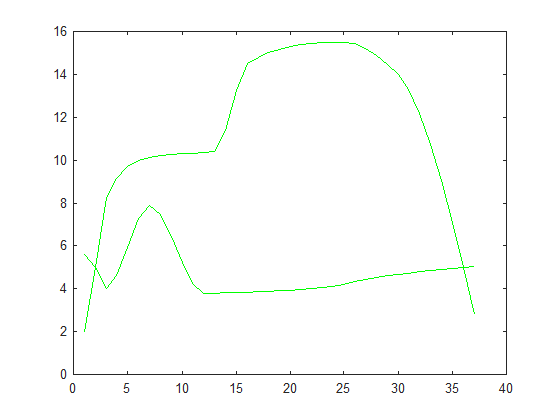
\includegraphics[width=9cm]{interp_spline_csaps}
    \caption{interpolación Spline cubica suavizante.} \label{fig:interp_spline_csaps}
\end{figure}
\newpage
La función utilizada es:
 
\begin{itemize}
\item interp
\end{itemize}
obs: en esta función se puede cambiar el comando ya sea por spline,csaps u otras, así se ve su comportamiento en cada caso.
\item Como podría utilizar el polinomio de interpolación de Lagrange para aproximar la parte inferior del contorno del auto? Trace el grafico que obtiene en esta aproximación.

Primero, para plantear el uso del polinomio de interpolación de Lagrange se hará uso de la definición de este polinomio interporlante la cual se planteará a continuación.

 \begin{equation}
 p(x)=\sum_{i=0}^n yi*Li(x)
\end{equation}
\\ De lo anterior, se define inmediatamente el valor de Li de la siguiente manera:
 \begin{equation}
 Lk(x)=\prod_{j=0,j\not=k}^{n}
\end{equation}
Luego, despues de definir como se utilizará el polinimio interpolante de Lagrange, se aplica el algoritmo en MATLAB con el fin de obtener graficamente lo que se plantea. 
\begin{figure}[H]
    \centering
    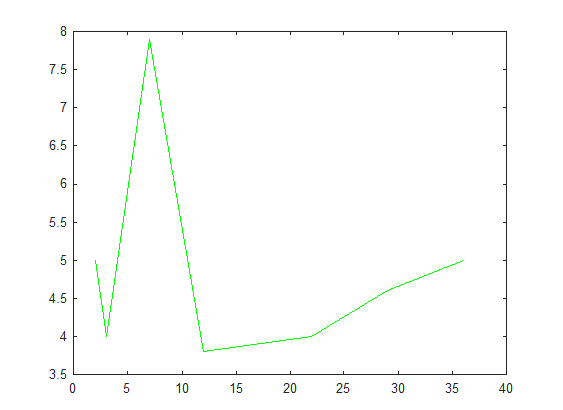
\includegraphics[width=9cm]{int_lagrange_inf}
    \caption{interpolación Lagrange parte inferior de auto.} \label{fig:int_lagrange_inf}
\end{figure}
Usando la misma interpolación polinómica de Lagrange y bajo el mismo algoritmo se grafica igualmente la parte superior del auto en cuestión.
\begin{figure}[H]
    \centering
    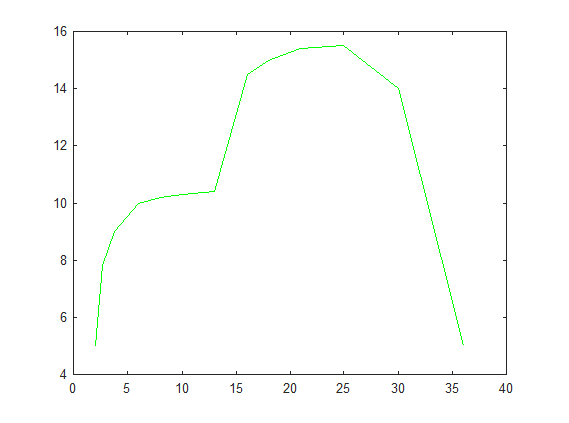
\includegraphics[width=9cm]{int_lagrange_aprox_parte_sup}
    \caption{interpolación lagrange parte superior de auto.} \label{fig:int_lagrange_aprox_parte_sup}
\end{figure}
La función utilizada es:
 
\begin{itemize}
\item lagrang(función que realiza el polinimio int)
\item lagrange(script que pide los datos)
\end{itemize}

\newpage


  
 \chapter{Integración de funciones} 

 
\begin{enumerate}
\item Corriente arriba de una presa, el agua ejerce una presión  P  y ejercida a una elevación z metros por encima del fondo fluvial. Si se omite la presión atmosférica, la fuerza puede ser determinada al multiplicar la presión por el  área de la cara de la presa. Esta área se obtiene integrando la función w (z) que proporciona el ancho del rio a una altura z del lecho y toma valores según la figura:
\end{enumerate}

 
 \begin{figure}[H]
    \centering
    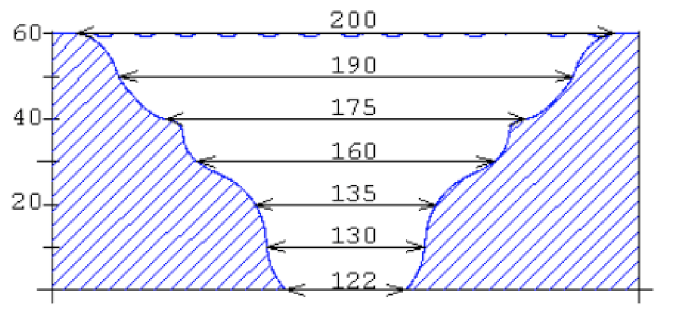
\includegraphics[width=9cm]{enunciado2}
    \caption{Ancho del rio W, respecto a la altura z.} \label{fig:enunciado2}
\end{figure}
Debido a que la presión y el área varan con la elevación, la fuerza total se obtiene al calcular
 \begin{equation}
 f=\int_{z=0}^{z=D} w(z)*(D-z) \cdot dz
\end{equation}
Donde (4) y (5) son la densidad del agua y la aceleración de gravedad, respectivamente. Por ultimo, D=60 que indica la elevación en metros.
\begin{equation}
 \rho=10^3[kg/m^3] 
\end{equation}
 
\begin{equation}
g=9.8[m/s^2]
\end{equation}
\\
 \begin{enumerate}
 \item Use la fórmula del trapecio compuesta (para 6 subintervalos) para calcular la fuerza total ejercida por el agua en la cara de la presa.
 \\ 
 \\
 Usando la fórmula del trapecio compuesto se obtiene que la fuerza total ejercida por el agua en la cara de la presa es la siguiente:
 \\
 \\
 f=1.0854e+10
\newpage
 El grafico obtenido en el proceso de obtención de la fuerza obtenida resultó ser la siguiente imagen.
 \begin{figure}[H]
    \centering
    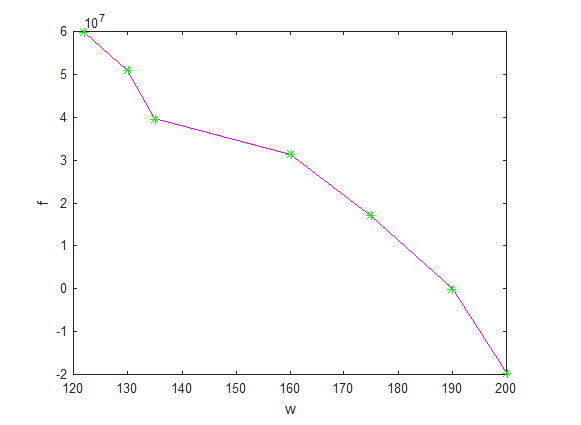
\includegraphics[width=9cm]{fuerza_trap}
    \caption{fuerza o presión en cada tramo calculado.} \label{fig:fuerza_trap}
\end{figure}
 \begin{figure}[H]
    \centering
    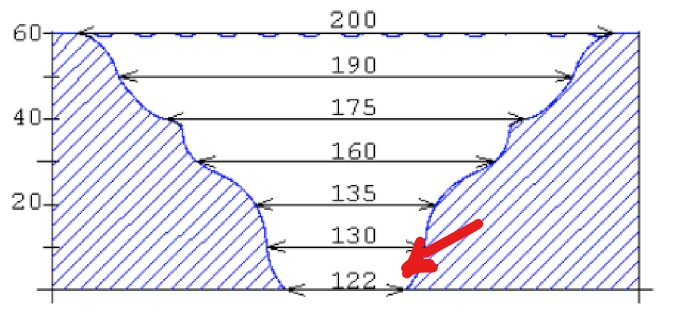
\includegraphics[width=9cm]{presionfin}
    \caption{presión en cota a mayor profundidad.} \label{fig:presionfin}
\end{figure}
Este gráfico e imagen indican que al estar en la cota que esta a mayor profundidad tal como lo muestra la figura 8 (espaciado 122 metros entre las caras de la presa) se ejerce una mayor fuerza perpendicular, esto quiere decir que el analisis realizado esta cercano a lo real ya que cumple con los principios fundamentales de la hidrostática. 
La función utilizada es:
 
\begin{itemize}
\item trapecio
\end{itemize}

 \vspace{0.8cm}
 
 \item Usando interpolación de Lagrange, dibuje la curva del lado derecho de la  figura.
 
  \begin{figure}[H]
    \centering
    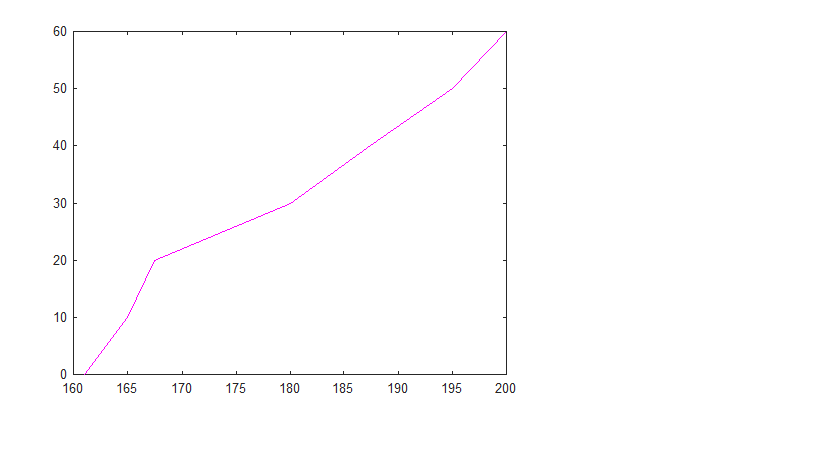
\includegraphics[width=9cm]{curva_derecha_lagrange}
    \caption{Curva lado derecho de la presa, interpolación polinómica de Lagrange.} \label{fig:curva_derecha_lagrange}
  
\end{figure}
\begin{itemize}
\item lagrang
\item lagrange
\end{itemize}
\newpage
 \item Usando interpolación por spline, dibuje la curva del lado izquierdo de la  figura.
 \\
 \begin{figure}[H]
    \centering
    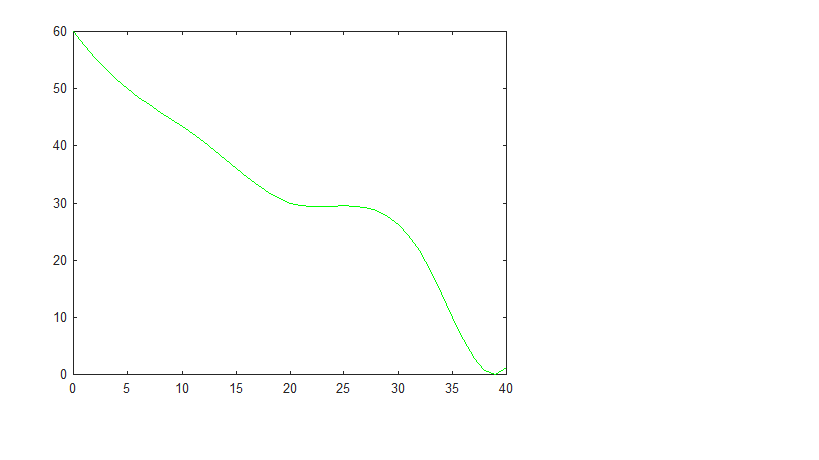
\includegraphics[width=9cm]{curvaizq_spline}
    \caption{Curva lado izquierdo de la presa, interpolación por spline cubico.} \label{fig:curvaizq_spline}
\end{figure}
\begin{itemize}
\item nuevospline
\end{itemize}
 \end{enumerate}
 \end{enumerate}

 \newpage

    
    
\chapter{Conclusión}
Del trabajo realizado durante este informe se concluye que principalmente se cumplen con los objetivos fundamentales planteados en la introducción,  primero, para la resolución de sistemas lineales, el uso de factorizaciones como por ejemplo la de Cholesky fue fundamental para encontrar la solución de un sistema matricial AX=B, de este mismo sistema se puede obtener el numero condición de la matriz A de dicho sistema, eso con el fin de ver si está bien condicionada o no.
\\
Otro punto a destacar fue el uso de métodos iterativos como Richardson, Jacobi, Gauss-Seidel y relajación para obtener la distribución inicial de mensajes en servidores con determinada distribución de probabilidad de Poisson.
\\
Con respecto a la aproximación de funciones, de forma general se puede afirmar que el uso de la interpolación Spline es más cercana a aproximar el contorno del auto lo más cercano a la imagen original en comparación a la interpolación polinómica de Lagrange, esto se pudo deber posiblemente a algún error en la programación del algoritmo planteado, eso sí , es importante decir que la aproximación de Lagrange fue menos exacta en la parte inferior del auto que en la parte exterior, es decir, al aproximar la parte exterior del auto fue muy similar tanto Lagrange como Spline cubico. 
\\
Finalmente, en la parte donde se muestra una presa, lo central de este problema fue obtener la presión sobre las paredes de dicha presa ejercidas por la corriente de agua. Al aplicar la fórmula del trapecio compuesto, se van adhiriendo por intervalos en determinadas alturas las fuerzas que se ejercen sobre las paredes de esta presa, la finalidad de esta sección es demostrar los principios de la hidrostática que plantean a grandes rasgos que a mayor profundidad, la fuerza que se ejerce en las paredes contenedoras es mucho mayor y perpendicular a estas.


\end{document}
